\documentclass[conference, a4paper, 10pt, twocolumn]{IEEEtran}
\usepackage{amsmath,amssymb,amsfonts}
\usepackage{algorithmic}
\usepackage{graphicx}
\usepackage{textcomp}
\usepackage{xcolor}
\usepackage{acronym}
\usepackage[style=ieee]{biblatex}
\usepackage[nottoc]{tocbibind}
\def\BibTeX{{\rm B\kern-.05em{\sc i\kern-.025em b}\kern-.08em
    T\kern-.1667em\lower.7ex\hbox{E}\kern-.125emX}}

\addbibresource{literature_list.bib}
\renewcommand*{\bibfont}{\small}

\newacro{API} {\textit{Application Programming Interface}}

\begin{document}

\title{Mechanisms to Raise Awareness about Smartwatch Data Collection}

\author{
	\IEEEauthorblockN{
		Mehmed Mustafa
	}
	\IEEEauthorblockA{
		\textit{Institute of Computer Science}\\
		\textit{University of G\"{o}ttingen}\\
		G\"{o}ttingen, Germany\\
		Email: mehmed.mustafa@stud.uni-goettingen.de
	}
	\and
	\IEEEauthorblockN{
		Chris Warin
	}
	\IEEEauthorblockA{
		\textit{Institute of Computer Science}\\
		\textit{University of G\"{o}ttingen}\\
		G\"{o}ttingen, Germany\\
		Email: chris.warin@stud.uni-goettingen.de
	}
}

\maketitle
\thispagestyle{plain}
\pagestyle{plain}


\begin{abstract}
This document is a model and instructions for \LaTeX.
This and the IEEEtran.cls file define the components of your paper [title, text, heads, etc.]. *CRITICAL: Do Not Use Symbols, Special Characters, Footnotes, 
or Math in Paper Title or Abstract.
\end{abstract}

\begin{IEEEkeywords}
component, formatting, style, styling, insert
\end{IEEEkeywords}

\section{Introduction}

\section{Foundations}\label{foundations}

The main goal of our work is to raise the awareness about smartwatch data collection. In this section, we first clarify our notion of smartwatch data collection and describe the technologies and platforms we use. 

A smartwatch is a device in the form of a watch which has computing capabilities. Although the earlier models had restricted functionality, the models starting from early 2010s are closer to smartphones in regard to features. Modern smartwatches have WiFi/Bluetooth connectivity, support mobile apps, have their own operating system and peripheral devices, which may include health tracking sensors such as heart rate monitors, location tracking sensors such as GPS receivers and activity tracking sensors such as pedometers.\cite{smartwatchWiki}

Mobile apps may gather data from different sensors at any given time. We refer to this process as smartwatch data collection. Mobile apps often ask the permission to use different sensors when they are launched for the first time. Users give permission but are not aware of exactly when and how often apps gather, e.g., their health, location or activity data. We propose 3 different mechanisms to increase the awareness users about the data gathering process: Visual, Sound and Haptic feedback. The visual feedback divides into 3 sub categories: Ring, Icon and Notification. The awareness increasing mechanisms are discussed in more details in section \ref{approach}. Our proposal could be further extended and developed as an API which developers could use in the future.

\begin{figure}[t]
\leftline{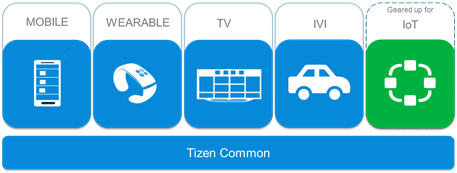
\includegraphics[width=.5\textwidth]{img/tizenInfrastructure.png}}
\caption{Tizen infrastructure}
\label{fig:tizen}
\end{figure}

For our research, we used a Samsung Galaxy Watch 3 \cite{galaxyWatch3}. The smartwatch runs Tizen OS 5.5, an open source Linux-based mobile operating system which is built to work on diverse devices. In order to support different types of devices and provide product-optimized performance, Tizen uses different profiles to categorize functions and features according to the requirements of each device type. Currently, four profiles are supported: IoT, Mobile, TV, and Wearable. Since all profiles are built on top of a common, shared infrastructure (as shown in Fig.~\ref{fig:tizen}), it is easy to add new profiles for emerging technologies \cite{tizen}.

% ref for Fig. 1

Tizen has its own official IDE for developing web based and native applications. Moreover, the availability of Tizen extensions for the Visual Studio Family makes possible to develop Tizen applications in the .NET environment. Tizen .NET, in comparison to web and native frameworks, is more advantageous. The C-based framework does not have advantages of a managed runtime and the HTML5-based framework has fewer features supported and worse performance. On the other hand, Tizen .NET has managed runtime advantages such as faster development, safer code, cross-platform support and better quality software. Tizen provides an emulator which increases the application development process. Firstly, because we do not need an actual physical device to start the development process. And secondly, because the control panel of the emulator makes it possible to produce different sensor values \cite{tizen}.


\section{Related Work}\label{related}

\section{Approach}\label{approach}

\section{Discussion}\label{discussion}
This section discusses the different approaches that were used in order to raise awareness in smartwatch data collection. Prior to developping the application that was discussed in section \ref{approach}, we imagined another application that was, to the best of our knowledge, not realizable with current \acp{API} and system accesses.  

\subsection{First approach}
The first application that we attempted to develop relied on a monitoring mechanism that would detect any sensor usage by another application that is installed on the watch. This way, the application would have been able to alert the user when an application that they chose to monitor would have started sensing. Unfortunately, this approach was impossible to implement, although the necessary data for its functioning are existing.

In order to implement the mechanism, three pieces of information would have been necessary: (1) the time at which a sensor was accessed by an application, (2) the name of the requested sensor, and (3) the process ID of the application that requested the sensor. We thought about two possible ways of obtaining this information: first, through the .NET Standard \ac{API} - and by extention, Samsung's .NET \ac{API} that contains platform-specific functionalities\cite{tizen}. However, upon a thorough inspection of the documentation, we came to the conclusion that these \acp{API} do not provide methods to access sensors in a global context. This means that although it is possible to create instances of the \textbf{Sensor} class, these instances are only related to the context of the application. In other words, it is only possible to know whether a sensor is being accessed by the current application, but not by others. 

The second way to obtain the necessary information was to read the system log. This log contains all necessary data; as such, parsing it would allow the application to detect when a certain application reads a given sensor. Unfortunately, this idea also led to a dead end: although the system log is writable by any application, it is not made readable by the vendor. This is certainly for a security reason, as an application that can both read and write the log could impersonate another application. Currently, the log is only readable through the development bridge that is provided by Tizen. As such, the only way to read the log of a smartwatch is to have a nearby computer with the required tools, which made our implementation impossible for a standalone application on a smartwatch. An alternative to this would be gaining root access to access the log from the smartwatch, in a similar fashion as on Android devices. However, there are, to this day, no accessible ways to achieve this. Furthermore, even if there were, this would result in a non-accessible application, as we assume that most smartwatch users would not go through the hassle of rooting their device, especially not to obtain feedback about sensor usage. 

%Lack of Tizen documentation details - app_context_h - structure data -> not possible to peek and see what is this abstract data structure constructed from - in Native app

These dead-ends point at the lack of sensor data access, and eventually, at feedback mechanisms by smartwatch vendors and the Tizen platform. The only sensor related feedback offered by the smartwatch we used for development (Samsung Galaxy Watch 3) is the green light that blinks when the heart rate monitor is turned on---and it is not even a voluntary feedback given by the vendor, but a necessary light to calculate the heart rate of the user. Although it would be best if smartwatch vendors provided native mechanisms to raise awareness in sensor data collection, a good start would be for them to extend their \acp{API} in order to know if sensors are used by other applications. This would allow the development of applications similar to our first approach that could seduce users. As of today, we come to the conclusion that smartwatch application developers have to implement these mechanisms themselves like we did in our second approach.

\subsection{Second approach}
The impossibility to implement our first approach led us to start again from scratch, and develop the application described in section \ref{approach}. Although it is less generic than our first approach---in the sense that it can only give feedback related to sensors that it senses itself---it still offers functionalities that benefit users, but also potentially developers that want to create transparent applications regarding sensor data collection.

Firstly, our main application provides a good granularity of feedback for the user, in the sense that the three different types of visual feedback that the user can choose attract attention with a different intensity: the icons are more discreet than the blinking rings, which are in turn more discreet than the system notifications, which attract the most attention with a colorful cue, a long vibration and a loud sound. This can further be tuned with options to add vibration, sound, or both to the ring or icon visual feedbacks (the notification type already comes with its own sound and vibration). As a result, different combinations can be made to obtain various amounts and intensities of feedback, which can suit different kinds of users. For example, users that are interested in knowing when their smartwatch sensors are being used by the application but do not want to be constantly reminded can use the ring or icon visual feedback types without sound or vibration. This way, they will only notice sensor usage when they look at their watch and see visual feedback on the watch face. Similarly, users who want more knowledge and control on sensor usage can either use the notification feedback type, or add vibration and sound to the ring or icon visual feedback types. Adding sound or vibrations provides more active feedback as they attract the user's attention even when they are not looking at their smartwatch. 

Secondly, the sensor suspension mechanism empowers the user by letting them choose when and for how long the application will not read sensor data. Along with providing them control, this can also reassure them regarding transparency: they know that the application will not collect their personal data as they will not get any feedback. Furthermore, the empowering of users in this matter can also come from the previously mentioned granularity of feedback, as the users can adjust the amount and intensity of feedback to their liking. Gaining control over the collection and having choice over the feedback can put the user in a position where they no longer feel overwhelmed by the pervasiveness of technology.

% see if this can be tied to human in the loop lecture from usable security - a ref would be great as this is only assumptions we do since we have no study to prove our point 

Lastly, the design of our application is advantageous for future work and other developers. Our implementation relies on a communication between the main application, which does the sensing, and a watch face, that displays feedback upon receiving messages from the main application. The communication between the two components is made using the .NET \ac{API}. As a result, it would be possible to release the source code for the watch face component, along with an easy to follow documentation to indicate how to communicate with it. This way, developers could easily reuse the watch face and connect it to their own application.

Although our approach has several advantages, it also has its limits. The first one is that it is a mere prototype, in the sense that it is not a realistic application that could be released on the vendor's store. The application only randomly accesses the smartwatch sensors at random times, which is likely not how a realistic application would behave. This is, however, not an important point when considering how to raise awareness for data collection---the point of this application is rather to consider the efficiency of feedback that is related to sensor data.  

Another limit of this implementation is the application performance: during the development, we found that the smartwatch battery was depleting fastly, implying a heavy resource consumption from our application. This can be improved over time by getting a better understanding of the platform and therefore apply the best practices that the vendor recommends. Indeed, the .NET variant offered by Tizen, as opposed to the native and web variants, relies on various components from different entities: the .NET framework \ref{dotnet} is maintained by Microsoft, as well as the cross-platform UI framework Xamarin.Forms \ref{xamarin}. On top of this comes CircularUI \ref{circularUI}, which is maintained by Samsung and extends Xamarin.Forms for Samsung-specific hardware. Lastly, in a similar fashion, Samsung extends the .NET \ac{API} with TizenFX\ref{tizenFX} for hardware specific methods that are not covered by the base framework. All these components imply different documentations, which sometimes contradict each other, or are outdated. This makes it hard to fully understand the Tizen ecosystem and, therefore, to program efficiently for it. However, this limit can also be discarded when considering awareness for sensor data collection.

Lastly, our implementation can easily be bypassed by the user, if they simply chose to close or not run the main application. It would then not access any sensor until the user launched the application again. When considering a real-life case, it is probable that developers would put the sensor access logic in services applications that run in background. This would, however, raise the necessity to ensure that such background services could be stopped when the data they gather is outside the scope of the purpose for which they are collected. For example, if we consider a scenario where a company provides its employees with an internal application that collects sensor data (e.g. to assess the employees' wellness), then such an application should not be allowed to sense data outside of working hours. Regardless, this limitation is rather related to the platform than the problem of raising awareness. 

Globally, none of the limitations of our current approach are critical when considering mechanisms to raise awareness in smartwatch data collection. However, the impossibility to implement the first one is in itself the major limit that prevented us from going further into this more global direction of providing feedback in a general way for all sensor accesses---not just the current application.

\section{Conclusion}
This report presented our proposal for mechanisms that raise awareness about smartwatch data collection. An overview of the capabilities of current smartwatches and their systems is described is section \ref{foundations}. We compared our work with past litterature. On one hand, there is evidence about users' privacy concerns when it comes to smartwatch devices \ref{}. On the other hand, there are various proposal of systems that give feedback to users for various usages, such as medical, or more recently, hygienic \ref{}. However, these two fields are, to the best of our knowledge, not connected together. As such, we are not aware of mechanisms that give users feedback related to data collection in smartwatches. 

Given this, we attempted to create a monitoring application that could detect when installed applications access sensors, and give feedback accordingly. This attempt resulted in failure, due to the lack of tools to achieve our goal. This result hopefully points out at the necessity for vendors to provide \acp{API} that can indicate sensor usage in a global context instead of restricting it to the app context only. 

From this, we implemented a prototype application that sends various types and combinations of feedback to the user when it accesses smartwartch sensors, including visual, haptic and sonor feedback. The application is divided between a watch face (i.e. the main interface of a smartwatch which mainly displays the time among other things; here, visual feedback) an a main application which accesses sensors and sends messages to the watch face. The main application also supports user preferences: the user can choose between different visual feedbacks and whether they want to add sounds or vibration on top of the visual feedback. These diferent combinations allow for a wide granularity of feedback, which can better suit users depending on the amount of feedback they want. Furthermore, users are put in control through a sensor suspension mechanism: they can set a timer until which the application can not access any sensor. Globally, this approach should both reassure users when they do not perceive any feedback (because this implies no collection of their data) and raise their awareness when the feedback informs them of data colleciton.  

The interest for this project is that it mimicks what a real-life application could do. Considering a scenario where a company provides its employees with an application that collects sensor data in a transparent way (i.e. by giving corresponding feedback) justifies our application in the sense that this could be the next step for smartwatch applications in the future. Furthermore, the watch face code could be shared to the Tizen community as a first step towards a global \ac{API}. As such, having groundwork in this direction is of importance.


\begin{figure*}[ht]
\centerline{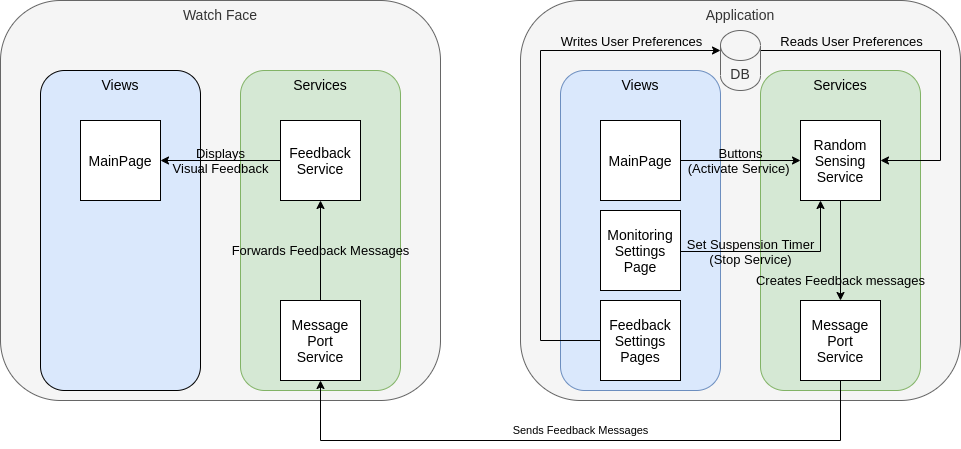
\includegraphics[width=1\textwidth]{img/appDiagram.png}}
\caption{Example of a figure caption.}
\label{fig}
\end{figure*}

\section*{Acknowledgment}

\printbibliography

\end{document}
